\chapter{Simulationsergebnisse}\label{ch:Simulationsergebniss}

Die Abbildung \ref{fig:Doppelpendel_Ergebniss_Simulink} zeigt die Ergebnisse der Simulation des Doppelpendels in Simulink mit 5-Punkte Schema. Die Simulation wurde mit den Parametern $l_1 = 0,2~m$, $l_2 = 0,2~m$, $m_1 = 0,0295~kg$, $m_2 = 0,0295~kg$ und $s_1 = 0,1~m$, $s_2 = 0,1~m$, $J_1 = 9,8175 \cdot 10^{-5}~kg \cdot m^2$, $J_2 = 9,8175 \cdot 10^{-5}~kg \cdot m^2$ durchgeführt. Die Anfangswerte für die Winkel wurden auf $\varphi_1 = 0~rad$ und $\varphi_2 = \pi/2~rad$ gesetzt. Die Simulation wurde über einen Zeitraum von $10~sec$ durchgeführt.
\begin{figure}[H]
    \centering
    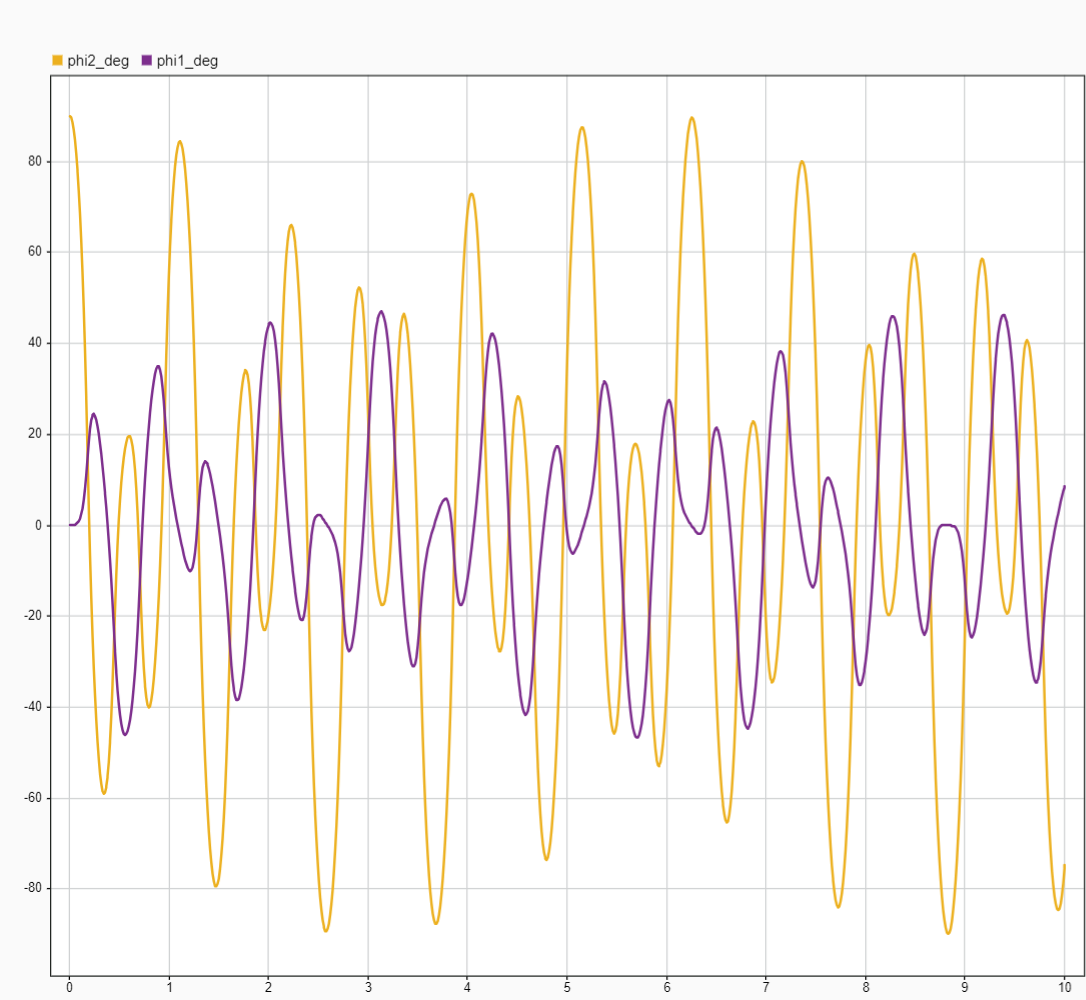
\includegraphics[width=0.45\textwidth]{figures/Doppelpendel_Ergebniss_Simulink.png}
    \caption{Doppelpendel Ergebniss mit 5-Punkte Schema}
    \label{fig:Doppelpendel_Ergebniss_Simulink}
\end{figure}

Die Abbildung \ref{fig:Doppelpendel_Ergebniss_Zustandsraum} zeigt die Ergebnisse der Simulation des Doppelpendels mit Zustandsraummodell. Die Simulation wurde mit den gleichen Parametern und Anfangsbedingungen wie die Simulation mit 5-Punkte Schema durchgeführt. Nach Linearisierung des Modells sieht die die Ergebnisse ähnlich aber nicht gleich wie die Ergebnisse der Simulation mit 5-Punkte Schema. 
\begin{figure}[H]
  \centering
  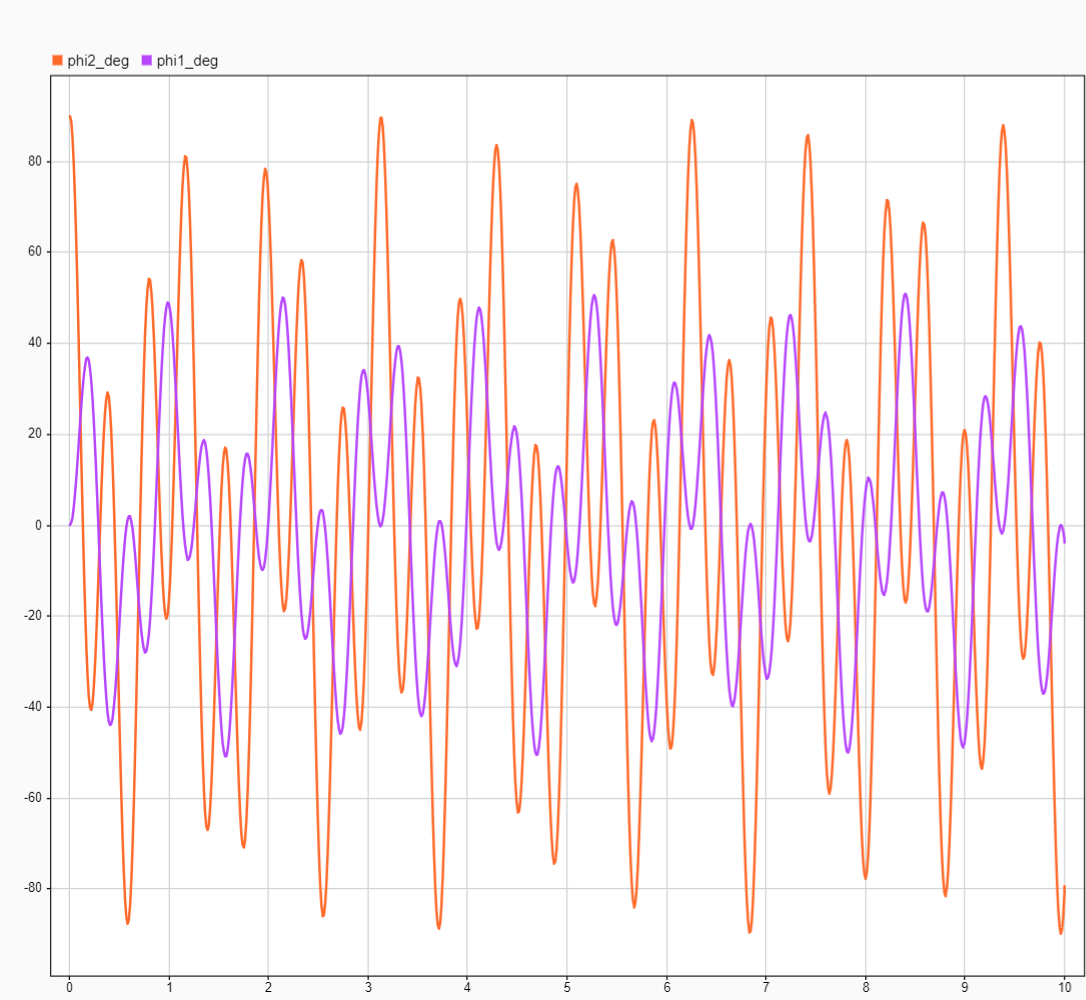
\includegraphics[width=0.45\textwidth]{figures/Doppelpendel_Ergebniss_Zustandsraum.png}
  \caption{Doppelpendel Ergebniss mit Zustandsraummodell}
  \label{fig:Doppelpendel_Ergebniss_Zustandsraum}
\end{figure}

Folgende Abbildung \ref{fig:Doppelpendel_Ergebniss} zeigt die Ergebnisse der Simulation des Doppelpendels in Matlab (ohne Simulink). Die Simulation wurde mit den gleichen Parametern und Anfangsbedingungen wie die Simulation in Simulink durchgeführt. Die Ergebnisse zeigen, dass die Simulation in Matlab fast gleiche Ergebnisse wie die Simulation in Simulink mit 5-Punkte Schema liefert. 
\begin{figure}[H]
    \centering
    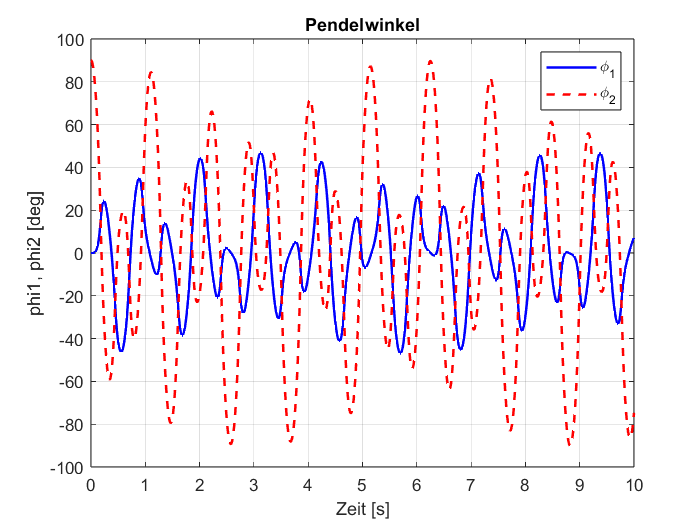
\includegraphics[width=0.6\textwidth]{figures/Doppelpendel_Ergebniss.png}
    \caption{Doppelpendel Ergebniss in Matlab (ohne Simulink)}
    \label{fig:Doppelpendel_Ergebniss}
\end{figure}

Für Erweiterungen simuliert hier ein Dreifachpendel mit Matlab (ohne Simulink). Die Abbildung \ref{fig:Dreifachpendel_Ergebniss} zeigt die Ergebnisse der Simulation des Dreifachpendels. Die Simulation wurde mit gleiche Parametern und wie das Doppelpendel durchgeführt. Die Anfangswerte für die Winkel wurden auf $\varphi_1 = 0~rad$, $\varphi_2 = 0~rad$ und $\varphi_3 = \pi/2~rad$ gesetzt. Die Abbildung \ref{fig:Dreifachpendel_Ergebniss_Trajektorie} zeigt die Trajektorie der dritten Pendel in der Simulation des Dreifachpendels.
\begin{figure}[H]
    \centering
    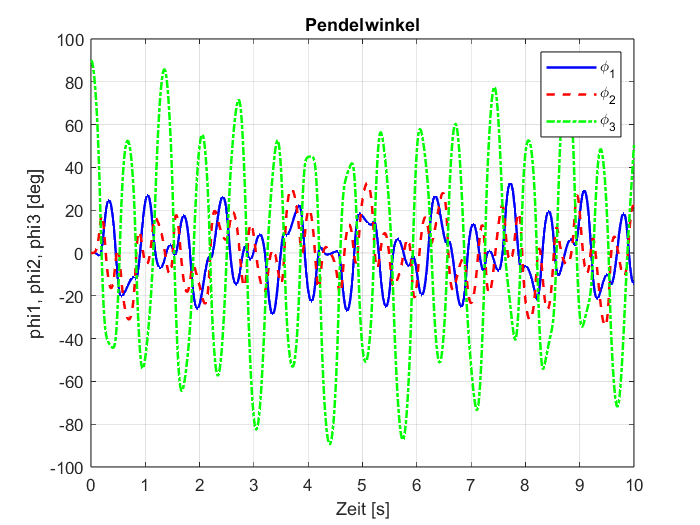
\includegraphics[width=0.6\textwidth]{figures/Dreifachpendel_Ergebniss.png}
    \caption{Dreifachpendel Ergebniss in Matlab (ohne Simulink)}
    \label{fig:Dreifachpendel_Ergebniss}
  \end{figure}

\begin{figure}[H]
    \centering
    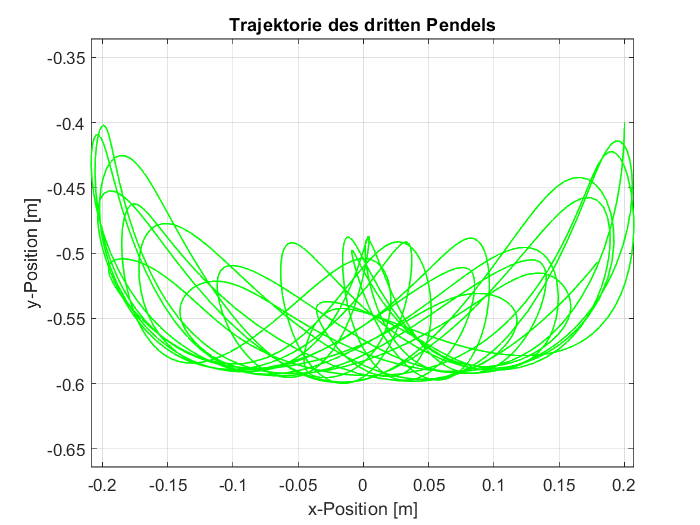
\includegraphics[width=0.6\textwidth]{figures/Dreifachpendel_Ergebniss_Trajektorie.png}
    \caption{Trajektorie von dritten Pendel des Dreifachpendels}
    \label{fig:Dreifachpendel_Ergebniss_Trajektorie}
\end{figure}

Die Ergebnisse der Simulation zeigen, dass das Doppelpendel und das Dreifachpendel chaotisches Verhalten aufweisen. Beide Methoden (Matlab und Simulink mit 5-Punkte Schema) liefern ähnliche Ergebnisse, wobei die Simulation mit Zustandsraummodell eine gewisse Abweichung aufweist. Der Grund für diese Abweichung könnte in der Linearisierung des Modells liegen, die nur in einem kleinen Bereich um den Gleichgewichtspunkt gültig ist. 

Zusammenfassend lässt sich sagen, dass die Simulation des Doppelpendels und des Dreifachpendels in Matlab und Simulink erfolgreich durchgeführt wurde. Die Ergebnisse bestätigen die theoretischen Annahmen über die Dynamik des Systems. Mit aktuellen Modellen und Methoden können in der Zukunft weitere Simulationen durchgeführt werden. Z.B. Regelung des Pendels mit PID-Regler oder Zustandsraumregelung. 